%% Chapter 4 — Specifications & Risk Prioritization
%% Course 247-519-VA, Vanier College
%% Project Planning & Prototyping

\chapter{Specifications \& Risk Prioritization}
\label{ch:specifications}

Chapter~3 produced two things: a precisely framed central question and a justified fidelity choice.
Those outputs identify \emph{what} must be true for the prototype to succeed, but they do not yet say \emph{how true} is true enough --- that gap is what a specification fills.
This chapter shows how to convert that central question into measurable, testable requirements and a ranked risk register --- the Stage-Gate Stage~2 Scoping deliverables --- by using two complementary tools: a simple risk equation and an FMEA-style Risk Priority Number.

By the end of this chapter you will be able to:
\begin{enumerate}
  \item write measurable, testable requirements that can unambiguously pass or fail;
  \item separate requirements (the \emph{what}) from design decisions (the \emph{how}); and
  \item build and defend a risk-priority ranking that guides prototype focus.
\end{enumerate}

% ─────────────────────────────────────────────────────────────────────────────
\section{Anatomy of a Specification}
\label{sec:ch4-anatomy}
% ─────────────────────────────────────────────────────────────────────────────

A \index{specification}specification is a contract between the engineering team and every stakeholder who must eventually verify the product.
It answers one question per line: \emph{how will we know we succeeded?}
A well-formed specification document contains five distinct element types, each serving a different verification role.

\subsection{Functional Requirements}
\label{subsec:ch4-functional}

A \index{functional requirement}functional requirement states a capability the system must provide, expressed as a verb phrase with a measurable threshold.
The threshold is what separates a functional requirement from a vague aspiration.

\begin{itemize}
  \item \textbf{Weak (untestable):} ``The system shall sort items quickly.''
  \item \textbf{Strong (testable):} ``The system shall classify and divert each item within $\leq$167~ms of entering the sensor gate (throughput $\geq$6~items/min, continuous 1-hour run).''
\end{itemize}

Every functional requirement must name: (a) the actor or subsystem, (b) the action, (c) the measurable threshold, and (d) the operating condition under which the threshold applies.

\subsection{Performance Targets}
\label{subsec:ch4-performance}

\index{performance target}Performance targets quantify quality-of-behaviour: accuracy, latency, bandwidth, efficiency.
They differ from functional requirements in that they govern \emph{how well} the function is performed, not merely \emph{whether} it is performed.
A sorter that classifies items at 6~items/min but with 40\% error satisfies the throughput functional requirement yet fails the accuracy performance target.

\subsection{Constraints}
\label{subsec:ch4-constraints}

\index{constraint}Constraints are non-negotiable boundaries imposed by physics, regulation, or business.
They do not describe desirable behaviour; they eliminate design options outright.
Examples: BOM cost $\leq$\$500~CAD (business constraint), supply voltage from USB $\leq$5~V at 2~A (interface constraint), operating temperature 0–50\textdegree{}C (environmental constraint).

\subsection{Interfaces}
\label{subsec:ch4-interfaces}

\index{interface specification}Interface specifications describe the boundaries between subsystems, between the product and external systems, and between the product and its users.
A \index{mechanical interface}mechanical interface names connector types and physical envelope; an \index{electrical interface}electrical interface names voltage levels, connector pinouts, and communication protocols; a \index{software interface}software interface names message formats, topics, and timing.
Specifying interfaces early prevents integration surprises — the most common source of late-stage schedule overrun.

\subsection{Acceptance Criteria}
\label{subsec:ch4-acceptance}

\index{acceptance criterion}Acceptance criteria translate every requirement into a concrete test: apparatus, procedure, pass/fail decision rule.
Writing the acceptance test at the same time as the requirement is a discipline check: if you cannot describe how to measure it, the requirement is not yet measurable.

\paragraph{In Practice.}
At Vanier's Product Development Lab, teams have learned to draft acceptance criteria as a three-column table: \emph{Requirement ID}, \emph{Test Procedure} (apparatus + steps), \emph{Pass Condition}.
Filling this table during Week~2 surfaces ambiguous requirements before any hardware is ordered, saving the cost of a redesign sprint.

% ─────────────────────────────────────────────────────────────────────────────
\section{Requirements vs.\ Design}
\label{sec:ch4-req-vs-design}
% ─────────────────────────────────────────────────────────────────────────────

\index{requirements vs.\ design}The single most persistent error in student (and professional) specification documents is embedding a design decision inside a requirement.
Figure~\ref{fig:ch4-req-vs-design} shows a side-by-side comparison of requirement and design statements for the same capability.

\begin{figure}[htbp]
  \centering
  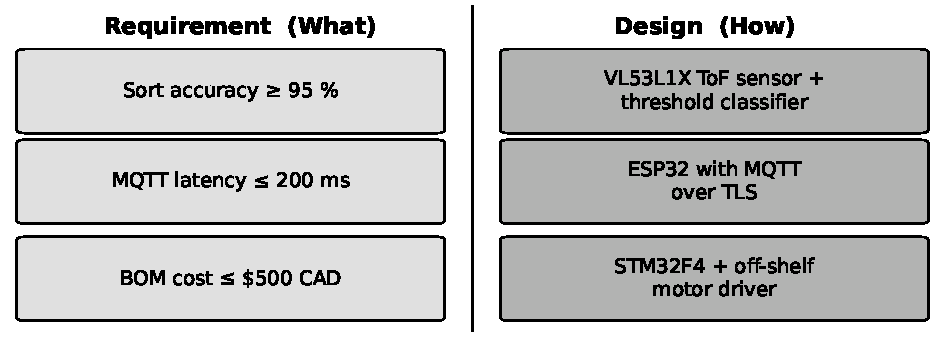
\includegraphics[width=0.85\textwidth]{images/fig_02_req_vs_design}
  \caption{Side-by-side comparison of a requirement statement (left) and a design statement (right) for the same capability.
           Requirements describe observable, measurable outcomes; design statements prescribe implementation choices.}
  \label{fig:ch4-req-vs-design}
\end{figure}

A useful \index{test for requirements}test: replace the specific implementation with an alternative one.
If the requirement is still meaningful, it is a genuine requirement.
If it becomes nonsensical, it was a design decision dressed up as a requirement.

\begin{itemize}
  \item \textbf{Requirement:} ``Classification results shall be transmitted to the cloud dashboard within $\leq$200~ms of each sort event.''
         Replacing Wi-Fi with Ethernet or cellular still leaves this requirement meaningful. \checkmark
  \item \textbf{Design-embedded (invalid):} ``The MCU shall use MQTT over Wi-Fi to transmit classification results.''
         This mandates the implementation, closing off alternatives before the team has evaluated trade-offs. \texttimes
\end{itemize}

\subsection{The ``What / How'' Discipline}
\label{subsec:ch4-what-how}

\index{what/how discipline}Every line of a specification document should survive the question: ``Does this describe what the system must do, or does it describe how we plan to do it?''
The \emph{what} belongs in the specification.
The \emph{how} belongs in the design document, the architecture diagram, or the BOM — produced \emph{after} requirements are frozen.

\paragraph{In Practice.}
When reviewing a teammate's specification draft, highlight every noun that names a specific component (``Arduino'', ``ToF sensor'', ``Python'') or a specific topology (``mesh network'', ``I\textsuperscript{2}C bus'').
Each highlighted phrase is a candidate design decision that may be pre-empting a better alternative.
Move it to the design rationale section and restate the requirement in terms of observable behaviour.

\paragraph{Common Pitfalls.}
\begin{itemize}
  \item \textbf{Unmeasurable criteria.} ``The system shall be user-friendly'' cannot be tested.
        Restate as: ``A first-time operator shall complete initial setup in $\leq$10~minutes following the Quick-Start card, with zero support calls, measured on five na\"{i}ve participants.''
  \item \textbf{Embedding the solution.} ``The sensor shall use a VL53L1X time-of-flight module'' is a design choice.
        The requirement should read: ``The sensor subsystem shall detect items up to 300~mm from the gate with $\leq$2~mm resolution at throughput $\geq$6~items/min.''
  \item \textbf{Ambiguous conditions.} A requirement with no stated operating condition is incomplete.
        ``Latency $\leq$200~ms'' must specify: under what network load? at what ambient temperature? for what message size?
\end{itemize}

% ─────────────────────────────────────────────────────────────────────────────
\section{Risk-Driven Prioritization}
\label{sec:ch4-risk-priority}
% ─────────────────────────────────────────────────────────────────────────────

\index{risk-driven prioritization}Once requirements exist, the team must decide which risks — failures to meet those requirements — deserve the most engineering attention.
Without a principled ranking, teams either (a) work on the most visible problem rather than the most dangerous one, or (b) try to mitigate everything simultaneously and mitigate nothing well.

\subsection{The Basic Risk Equation}
\label{subsec:ch4-risk-eq}

The simplest risk model assigns two quantities to each potential failure mode:

\begin{itemize}
  \item $P_{\text{failure}}$\index{probability of failure}: the estimated probability that the failure occurs in a prototype or field unit, scored 1–10 (1 = very unlikely, 10 = near-certain).
  \item $C_{\text{consequence}}$\index{consequence}: the estimated cost of that failure — in schedule days, dollars, or safety impact — scored 1–10 (1 = trivial, 10 = project-ending).
\end{itemize}

\begin{equation}
  R = P_{\text{failure}} \times C_{\text{consequence}}
  \label{eq:ch4-risk}
\end{equation}

The resulting risk score $R$ ranges from 1 to 100.
Teams typically set a threshold (e.g., $R \geq 30$) above which a mitigation plan is mandatory.
Figure~\ref{fig:ch4-risk-matrix} shows a probability–consequence matrix that maps risk scores to action zones.

\begin{figure}[htbp]
  \centering
  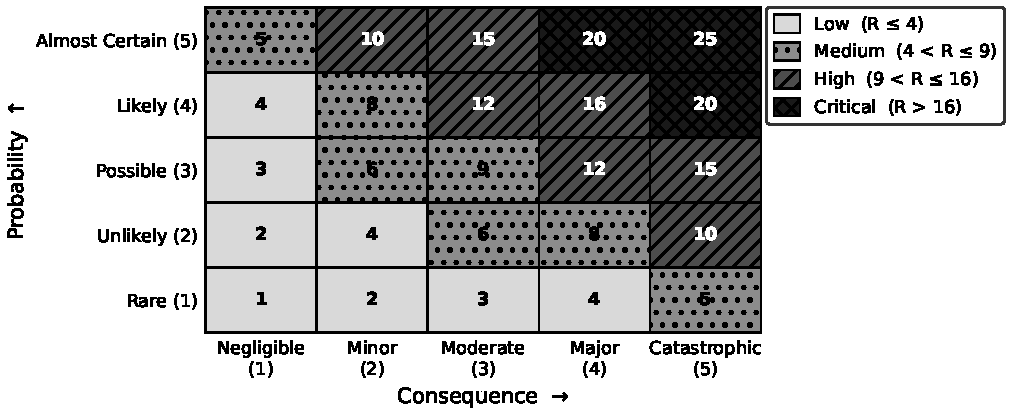
\includegraphics[width=0.85\textwidth]{images/fig_01_risk_matrix}
  \caption{Probability $\times$ consequence risk matrix for the running example.
           Cells with $R \geq 30$ fall in the red action zone; $15 \leq R < 30$ in the amber watch zone; $R < 15$ in the green monitor zone.}
  \label{fig:ch4-risk-matrix}
\end{figure}

\subsection{Limitations of the Two-Factor Model}
\label{subsec:ch4-risk-limits}

Equation~\eqref{eq:ch4-risk} is fast and easy to communicate to non-technical stakeholders, but it conflates two distinct ideas: the \emph{probability} that a failure reaches the user and the \emph{team's ability to detect} a failure before it causes harm.
A failure mode that is severe and somewhat likely but detectable in bench testing is far less dangerous than one that is equally severe but invisible until field deployment.
Section~\ref{sec:ch4-fmea} introduces the FMEA Risk Priority Number, which adds detection as a third factor.

% ─────────────────────────────────────────────────────────────────────────────
\section{FMEA-Style Ranking (RPN)}
\label{sec:ch4-fmea}
% ─────────────────────────────────────────────────────────────────────────────

\index{FMEA}\index{Failure Mode and Effects Analysis}Failure Mode and Effects Analysis (FMEA) is a structured method for systematically enumerating every way a system can fail, estimating three quantities for each failure mode, and computing a Risk Priority Number to guide mitigation effort.

\subsection{The RPN Formula}
\label{subsec:ch4-rpn-formula}

\begin{equation}
  \text{RPN} = S \cdot O \cdot D
  \label{eq:ch4-rpn}
\end{equation}

\noindent where:
\begin{itemize}
  \item $S$ = \index{severity}Severity (1–10): how bad is the consequence if the failure reaches the user?
  \item $O$ = \index{occurrence}Occurrence (1–10): how likely is the failure to occur during normal operation?
  \item $D$ = \index{detection}Detection (1–10): how difficult is it to detect the failure before it affects the user?
        \emph{Note: a higher D score means harder to detect.}
\end{itemize}

RPN ranges from 1 to 1{,}000.
Unlike the two-factor risk score $R$, the RPN captures the value of test coverage: a team that adds a robust bench test lowers $D$ and therefore lowers RPN even without changing the underlying design.

\paragraph{In Practice.}
Industry FMEA tables typically flag RPN $\geq 100$ as requiring a documented corrective action, and RPN $\geq 200$ as requiring a design change before release.
For a student prototype, a lighter threshold — flag RPN $\geq 80$ — is appropriate, because prototype runs are short and failures are recoverable.

\subsection{Scale Anchors}
\label{subsec:ch4-scale-anchors}

Table~\ref{tab:ch4-scale} gives representative scale anchors for S, O, and D as used in this course.
Teams should agree on anchors \emph{before} scoring to prevent rater drift.

\begin{table}[htbp]
  \centering
  \caption{Representative 10-point scale anchors for FMEA scoring in a prototype context.}
  \label{tab:ch4-scale}
  \begin{tabular}{@{}clll@{}}
    \toprule
    Score & Severity ($S$) & Occurrence ($O$) & Detection ($D$) \\
    \midrule
    1--2  & No user impact         & Rare ($<$1 in 1{,}000 runs)        & Immediately obvious; alarms fire \\
    3--4  & Minor degradation      & Occasional ($\sim$1 in 100 runs)   & Detectable by inspection or log  \\
    5--6  & Partial loss of function & Moderate ($\sim$1 in 20 runs)    & Detectable only with test setup  \\
    7--8  & Major loss of function & Frequent ($\sim$1 in 5 runs)       & Difficult; requires special tool  \\
    9--10 & Safety / total failure & Near-certain ($>$1 in 2 runs)     & Cannot be detected before impact \\
    \bottomrule
  \end{tabular}
\end{table}

% ─────────────────────────────────────────────────────────────────────────────
\section{The Critical Path of Unknowns}
\label{sec:ch4-critical-path}
% ─────────────────────────────────────────────────────────────────────────────

\index{critical path of unknowns}The risk register produced by FMEA answers \emph{which} risks are largest.
A separate but related question is \emph{which risks must be resolved first} — because some unknowns block progress on every other subsystem.
This is the critical path of unknowns.

Figure~\ref{fig:ch4-critical-unknowns} illustrates the assumption list and dependency arrows for the running example.
The highest-RPN item that \emph{also} blocks downstream work defines the prototype's first experiment.

\begin{figure}[htbp]
  \centering
  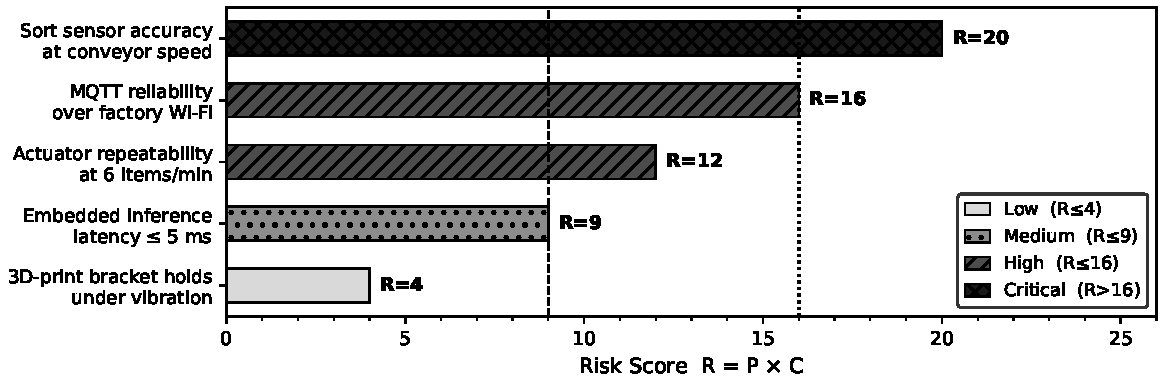
\includegraphics[width=0.85\textwidth]{images/fig_03_critical_unknowns}
  \caption{Critical unknowns and assumption dependency map for the IoT robotic sorting subsystem.
           Arrows show which assumptions must be resolved before dependent subsystem work can begin.
           The sort-sensor assumption (shaded) lies on the critical path because both the divert actuator timing and the firmware logic depend on its output format.}
  \label{fig:ch4-critical-unknowns}
\end{figure}

\subsection{Identifying the Critical Unknown}
\label{subsec:ch4-identify-critical}

To find the critical unknown, list every open assumption in the risk register and ask two questions for each:
\begin{enumerate}
  \item If this assumption turns out to be false, how many other subsystems must change? (Coupling score.)
  \item How quickly can we resolve it with a targeted experiment? (Resolvability score.)
\end{enumerate}

An assumption with high coupling and low resolvability is both dangerous and slow to clear — it should head the prototype schedule.
An assumption with high coupling but high resolvability should be the \emph{first} experiment run, because a quick test removes the blocker cheaply.

\paragraph{In Practice.}
For the IoT sorter, the sort-sensor detection principle (time-of-flight vs.\ break-beam vs.\ vision) is the critical unknown: the firmware state machine, the actuator timing, and the MQTT payload format all depend on what the sensor outputs.
Running a 48-hour bench test of candidate sensors \emph{before} ordering actuator parts avoids a costly mid-sprint pivot.

% ─────────────────────────────────────────────────────────────────────────────
\section{Worked Example: IoT Robotic Sorting Subsystem}
\label{sec:ch4-worked-example}
% ─────────────────────────────────────────────────────────────────────────────

This section walks through the full specification and risk-ranking workflow for the running example established in Chapter~3: a connected IoT robotic sorting subsystem classifying and diverting items on a bench conveyor, reporting over MQTT/Wi-Fi, with a target BOM of $\leq$\$500~CAD and a sort accuracy of $\geq$95\%.

\subsection{Step 1: Convert Vague Wishes into Measurable Requirements}
\label{subsec:ch4-step1}

The team's initial wish list contained five phrases typical of early ideation.
Table~\ref{tab:ch4-requirements} shows each vague phrase converted to a testable requirement.

The most instructive conversion is ``fast'':

\begin{itemize}
  \item \textbf{Vague:} ``The system shall process sensor data fast.''
  \item \textbf{Step 1 — name the quantity:} Processing speed is measured in samples per second (kS/s) and as end-to-end latency (ms).
  \item \textbf{Step 2 — anchor to the use case:} At 6~items/min, one item arrives every $60\,\text{s}/6 = 10\,\text{s}$.
        A single sort event reads one sensor frame, runs the classifier, and commands the actuator.
        The conveyor belt speed is 50~mm/s and the item window at the gate is 50~mm, giving a gate dwell time of $50\,\text{mm} \div 50\,\text{mm/s} = 1{,}000\,\text{ms}$.
        The actuator must fire within that window.
  \item \textbf{Step 3 — allocate the budget:}
        Budget allocation: sensor read 1~ms, classifier 2~ms, actuator command 2~ms, margin 995~ms.
        Conservatively, the end-to-end firmware latency budget is $\leq$5~ms.
        At a 10~kS/s ADC rate, the sensor delivers $10{,}000$ samples per second; one classification frame uses 10 samples, costing $10/10{,}000 = 1\,\text{ms}$ — within budget.
  \item \textbf{Measurable requirement:} ``The MCU firmware shall process one classification event (sensor read + classification + actuator command) within $\leq$5~ms, measured from sensor-trigger interrupt to actuator-enable GPIO, at a sustained rate of $\geq$10~kS/s sensor sampling.''
\end{itemize}

\begin{table}[htbp]
  \centering
  \caption{Vague feature wishes converted to measurable, testable requirements for the IoT robotic sorting subsystem.
           Each requirement identifies actor, action, threshold, and operating condition.}
  \label{tab:ch4-requirements}
  \begin{tabular}{@{}p{3.2cm}p{7.5cm}l@{}}
    \toprule
    Vague Wish & Measurable Requirement & ID \\
    \midrule
    ``Sorts accurately'' &
      The system shall classify items with $\geq$95\% accuracy (correct class / total items) over a continuous 100-item run at nominal belt speed. &
      REQ-01 \\[4pt]
    ``Fast'' &
      The MCU firmware shall complete one classification event within $\leq$5~ms (sensor read + classify + actuator command) at $\geq$10~kS/s sensor sampling. &
      REQ-02 \\[4pt]
    ``Enough throughput'' &
      The system shall sustain $\geq$6~items/min throughput for $\geq$60~min without thermal throttling or error accumulation. &
      REQ-03 \\[4pt]
    ``Sends data to the cloud'' &
      Each sort-event MQTT message shall be delivered to the broker within $\leq$200~ms of the sort event, on a 2.4~GHz Wi-Fi network with $\geq$-70~dBm RSSI. &
      REQ-04 \\[4pt]
    ``Affordable'' &
      The total prototype BOM (all purchased components) shall not exceed \$500~CAD. &
      REQ-05 \\
    \bottomrule
  \end{tabular}
\end{table}

A sixth implied constraint (power) is added from the hardware context:

\begin{itemize}
  \item[] \textbf{CON-01:} Total system power draw shall not exceed 5~W when powered from a single USB-C port (5~V, 2~A = 10~W; 5~W provides 50\% margin for host compatibility).
\end{itemize}

\subsection{Step 2: Compute RPN for Three Subsystems}
\label{subsec:ch4-step2}

The team identifies three high-risk subsystems from Chapter~3's prototype classification: (A)~Sort Sensor, (B)~MQTT/Wi-Fi Integration, (C)~Divert Actuator.
For each, the team identifies the primary failure mode, scores $S$, $O$, and $D$ on the 1–10 scale from Table~\ref{tab:ch4-scale}, and computes RPN using Equation~\eqref{eq:ch4-rpn}.

\bigskip
\noindent\textbf{Subsystem A — Sort Sensor}

\begin{itemize}
  \item \textbf{Failure mode:} Sensor misclassifies item class (false positive or false negative), causing a sort error.
  \item \textbf{Severity ($S$):} A miss ships a wrong item — significant product defect, customer complaint, possible recall. \textbf{$S = 8$}.
  \item \textbf{Occurrence ($O$):} Time-of-flight at $<$300~mm with a 50~mm/s belt is a moderately proven technique; reflectivity variation across item surface adds uncertainty. \textbf{$O = 5$}.
  \item \textbf{Detection ($D$):} A classification error is visible in the sort log and confirmed by counting missorted bins at end of run — easily detected during bench test. \textbf{$D = 2$}.
  \item \textbf{RPN:}
        \[
          \text{RPN}_A = S \cdot O \cdot D = 8 \times 5 \times 2 = \mathbf{80}
        \]
\end{itemize}

\noindent\textbf{Subsystem B — MQTT/Wi-Fi Integration}

\begin{itemize}
  \item \textbf{Failure mode:} MQTT message delivery latency exceeds 200~ms, causing dashboard staleness and potential missed alerts.
  \item \textbf{Severity ($S$):} Stale dashboard undermines the product's core value proposition (real-time visibility); does not stop physical sorting. \textbf{$S = 7$}.
  \item \textbf{Occurrence ($O$):} 2.4~GHz Wi-Fi in a lab environment with competing devices experiences frequent retransmissions; MQTT QoS~1 adds handshake overhead. \textbf{$O = 6$}.
  \item \textbf{Detection ($D$):} Latency can be measured by timestamping publish and subscribe events in the broker log — detectable but requires setup of a monitoring script. \textbf{$D = 4$}.
  \item \textbf{RPN:}
        \[
          \text{RPN}_B = S \cdot O \cdot D = 7 \times 6 \times 4 = \mathbf{168}
        \]
\end{itemize}

\noindent\textbf{Subsystem C — Divert Actuator}

\begin{itemize}
  \item \textbf{Failure mode:} Actuator fires too late or with insufficient force, failing to divert the item before it exits the gate.
  \item \textbf{Severity ($S$):} A missed divert is a sort error — same consequence as a sensor misclassification. \textbf{$S = 8$}.
  \item \textbf{Occurrence ($O$):} Servo or solenoid timing within a 1{,}000~ms dwell window is well within typical MCU PWM capability; mechanical linkage adds some uncertainty. \textbf{$O = 3$}.
  \item \textbf{Detection ($D$):} A missed divert is observable by watching the output bins or reading a secondary confirmation sensor — straightforward detection. \textbf{$D = 2$}.
  \item \textbf{RPN:}
        \[
          \text{RPN}_C = S \cdot O \cdot D = 8 \times 3 \times 2 = \mathbf{48}
        \]
\end{itemize}

\subsection{Step 3: Rank and Interpret}
\label{subsec:ch4-step3}

Table~\ref{tab:ch4-rpn} summarises the three RPN scores and maps each to a mitigation action.

\begin{table}[htbp]
  \centering
  \caption{FMEA Risk Priority Number ranking for the three prototype subsystems of the IoT robotic sorting subsystem.
           RPN computed using Equation~\eqref{eq:ch4-rpn}.
           Subsystems are sorted by descending RPN.}
  \label{tab:ch4-rpn}
  \begin{tabular}{@{}lllccccc@{}}
    \toprule
    Rank & Subsystem & Failure Mode & $S$ & $O$ & $D$ & RPN & Action \\
    \midrule
    1 & MQTT/Wi-Fi & Latency $>$200~ms  & 7 & 6 & 4 & \textbf{168} & Redesign / mitigate \\
    2 & Sort Sensor & Misclassification  & 8 & 5 & 2 & \textbf{80}  & Monitor / mitigate  \\
    3 & Divert Actuator & Late divert   & 8 & 3 & 2 & \textbf{48}  & Monitor             \\
    \bottomrule
  \end{tabular}
\end{table}

\noindent\textbf{Interpretation:}
\begin{itemize}
  \item MQTT/Wi-Fi integration (RPN = 168) is the highest-risk subsystem.
        The team should prototype and stress-test the Wi-Fi + MQTT stack \emph{first}, before investing time in actuator tuning.
        Concrete mitigation: run a dedicated latency characterisation script (publish 500 timestamped messages; record broker-side receive timestamp; compute 99th-percentile latency) within Sprint~1.
  \item Sort Sensor (RPN = 80) exceeds the 80-threshold and requires a documented mitigation plan.
        The sensor's detection principle should be confirmed in a 100-item accuracy trial before the firmware classifier is written.
  \item Divert Actuator (RPN = 48) is below the 80-threshold.
        Standard bench testing during integration is sufficient; no dedicated mitigation sprint is needed.
\end{itemize}

Applying the basic risk equation \eqref{eq:ch4-risk} for cross-check:
\begin{align*}
  R_A &= P_{\text{failure},A} \times C_{\text{consequence},A} = 5 \times 8 = 40 \quad (\text{action zone})\\
  R_B &= P_{\text{failure},B} \times C_{\text{consequence},B} = 6 \times 7 = 42 \quad (\text{action zone})\\
  R_C &= P_{\text{failure},C} \times C_{\text{consequence},C} = 3 \times 8 = 24 \quad (\text{watch zone})
\end{align*}

The two-factor scores \eqref{eq:ch4-risk} agree with the RPN ranking on the top item (MQTT/Wi-Fi) but obscure the gap between A and B that the detection factor ($D$) reveals.
The sensor is harder to detect as failing, so RPN correctly flags it above the threshold despite its lower occurrence rate.

% ─────────────────────────────────────────────────────────────────────────────
\subsection{Try It Yourself}
\label{subsec:ch4-try-it}
% ─────────────────────────────────────────────────────────────────────────────

\begin{quote}
\textbf{Scenario:} A team is developing a \textbf{smart irrigation controller} for a rooftop garden.
The system reads soil moisture via a capacitive sensor array, decides whether to open a motorised valve, and logs readings to a cloud dashboard over cellular (LTE-M).
The initial wish list contains:
\begin{itemize}
  \item ``Waters when needed'' — target: soil moisture sensor accuracy $\pm$3\% VWC
  \item ``Doesn't over-water'' — target: valve response within 30~s of a moisture threshold crossing
  \item ``Cheap to build'' — target: BOM $\leq$\$300~CAD
\end{itemize}

\textbf{Your tasks:}
\begin{enumerate}
  \item Rewrite each wish as a measurable requirement following the actor--action--threshold--condition format.
  \item Identify three failure modes (one per subsystem: moisture sensor, motorised valve, LTE-M uplink).
  \item Assign $S$, $O$, and $D$ scores on the 1–10 scale with written justification for each score.
  \item Compute RPN for each failure mode using Equation~\eqref{eq:ch4-rpn}, showing every multiplication step.
  \item Rank the three failure modes from highest to lowest RPN and state which subsystem should be prototyped first.
  \item Cross-check your top-ranked item using Equation~\eqref{eq:ch4-risk} and comment on whether the two rankings agree.
\end{enumerate}
Do \textbf{not} use the same S, O, D values as the worked example.
\end{quote}

% ─────────────────────────────────────────────────────────────────────────────
\section*{Review Questions}
\addcontentsline{toc}{section}{Review Questions}
\label{sec:ch4-review}
% ─────────────────────────────────────────────────────────────────────────────

\begin{enumerate}

  \item \textbf{(Conceptual)} Explain the difference between a \emph{functional requirement} and a \emph{performance target}, using one example of each from a product domain of your choice.
        Why must both be present in a complete specification?

  \item \textbf{(Conceptual)} A colleague argues that specifying the communication protocol (e.g., ``shall use Bluetooth Low Energy'') inside a requirement is efficient because it removes ambiguity for the firmware team.
        Justify why this practice is problematic and describe the correct place in the documentation hierarchy for such a decision.

  \item \textbf{(Applied — calculation)} A new IoT product team scores three failure modes as follows:
        \begin{itemize}
          \item Power regulator brown-out: $S = 9$, $O = 2$, $D = 3$
          \item Firmware deadlock: $S = 6$, $O = 7$, $D = 8$
          \item Enclosure latch failure: $S = 3$, $O = 4$, $D = 1$
        \end{itemize}
        Compute RPN for each failure mode using Equation~\eqref{eq:ch4-rpn}, showing every multiplication step.
        Rank them and state which subsystem requires a documented mitigation plan if the threshold is RPN $\geq 80$.

  \item \textbf{(Applied — multi-step calculation)} A wearable health monitor team sets an acceptance criterion: ``Heart-rate measurement error $\leq$3~BPM at 95\% confidence over a 10-minute walk test.''
        They estimate: $P_{\text{failure}} = 4$ (occasional out-of-range readings during vigorous movement), $C_{\text{consequence}} = 8$ (clinical misinterpretation risk).
        (a) Compute $R$ using Equation~\eqref{eq:ch4-risk}.
        (b) The team adds a real-time motion-artifact filter that lowers $O$ from 4 to 2.
            If $D$ remains at 3 and $S = 8$, compute the new RPN and state whether the mitigation moves the failure mode below threshold (Use Equation~\eqref{eq:ch4-rpn}).
        (c) Explain in one sentence why the two metrics ($R$ and RPN) give complementary information.

  \item \textbf{(Conceptual)} Define the \emph{critical path of unknowns} and explain how it differs from the highest-RPN item in the risk register.
        Give an example where the highest-RPN item is \emph{not} on the critical path of unknowns and describe what the team should do first.

\end{enumerate}

% ─────────────────────────────────────────────────────────────────────────────
\section*{End-of-Chapter Artifact}
\addcontentsline{toc}{section}{End-of-Chapter Artifact}
\label{sec:ch4-artifact}
% ─────────────────────────────────────────────────────────────────────────────

By completing this chapter's activities, you produce the core of \textbf{Milestone~1: the Proposal}.
The artifact has three interlocking parts:

\begin{enumerate}
  \item \textbf{Specification Table.}
        A table of 3–5 measurable requirements (functional requirements + performance targets) and any binding constraints, formatted with columns: ID, Requirement Statement, Threshold, Operating Condition, Acceptance Test.
        Each row must be testable as written.

  \item \textbf{Risk Register.}
        An FMEA table listing at least three failure modes (one per high-risk subsystem identified in Chapter~3).
        Each row contains: Subsystem, Failure Mode, $S$, $O$, $D$, RPN, Rank, and Mitigation Plan.
        The table is sorted by descending RPN.
        Failure modes above RPN~80 must have a specific mitigation action tied to a sprint.

  \item \textbf{Scoping Rationale.}
        One paragraph (100–150~words) that names: (a) the central prototype question, (b) the highest-risk assumption (the critical unknown), and (c) the first experiment that will resolve that assumption.
        This paragraph becomes the executive summary of your Milestone~1 submission.
\end{enumerate}

Together, these three parts answer the investor's foundational question: \emph{``What will this thing do, how will you know it works, and what could kill the project?''}

% ─────────────────────────────────────────────────────────────────────────────
\section*{Summary}
\addcontentsline{toc}{section}{Summary}
\label{sec:ch4-summary}
% ─────────────────────────────────────────────────────────────────────────────

This chapter introduced the anatomy of a specification — functional requirements, performance targets, constraints, interfaces, and acceptance criteria — and showed how each element must be measurable and testable.
It established the discipline of separating \emph{what} (requirements) from \emph{how} (design), a distinction that keeps early design choices from foreclosing better alternatives.
Two complementary risk tools were presented: the two-factor risk equation $R = P_{\text{failure}} \times C_{\text{consequence}}$ (Equation~\eqref{eq:ch4-risk}) for rapid stakeholder communication, and the FMEA Risk Priority Number $\text{RPN} = S \cdot O \cdot D$ (Equation~\eqref{eq:ch4-rpn}) for engineering-level prioritisation that accounts for detection difficulty.
Applied to the IoT robotic sorting subsystem, the analysis ranked MQTT/Wi-Fi integration (RPN = 168) as the first prototype target, followed by the sort sensor (RPN = 80), and confirmed that the divert actuator (RPN = 48) can proceed with standard integration testing.

You now have a specification table, a risk register, and a scoping rationale — the three components of the Milestone~1 Proposal.
Chapter~5 takes this artifact as its starting point and shows how to translate the highest-risk assumptions into a \emph{prototype plan}: selecting fidelity levels, designing the first experiment, and scheduling the sprint sequence that will resolve the critical unknowns in the right order.
